%!TEX root = ../../dissertation.tex
%%%%%%%%%%%%%%%%%%%%%%%%%%%%%%%%%%%%%%%%%%%%%%%%%%%%%%%%%%%%%%%%%%%%%%%%%%%%%%%%
%%%%%%%%%%%%%%%%%%%%%%%%%%%%%%%%%%%%%%%%%%%%%%%%%%%%%%%%%%%%%%%%%%%%%%%%%%%%%%%%
%%%%%%%%%%%%%%%%%%%%%%%%%%%%%%%%%%%%%%%%%%%%%%%%%%%%%%%%%%%%%%%%%%%%%%%%%%%%%%%%
\section{Background}
\label{c3:background}


%%%%%%%%%%%%%%%%%%%%%%%%%%%%%%%%%%%%%%%%%%%%%%%%%%%%%%%%%%%%%%%%%%%%%%%%%%%%%%%%
\subsection{Video Delivery Architecture}
\label{c3:sec:videodeliveryarchitecture}
Large Internet sites are not hosted at one central site anymore, but are usually served through geographically distributed entities forming a load-balancing structure. Such load balancing mechanisms have a long history on the Web, e.g. in the form of mirror servers a user can select manually.

In today's Content Distribution Networks (CDN), a much larger number of mirror servers is available, and selection of a server is no longer carried out explicitly by the user, but implicitly through DNS: Content is addressed using URLs (\texttt{http://somedomain/somepath} in its simplest form), and the CDN's DNS servers are configured to resolve certain domain names to different IP addresses, depending on where the query originated.

To get an insight into the structure of YouTube's content distribution network, we undertook a two-step measurement campaign \cite{rafetseder2011explyt}. First, we downloaded and manually parsed the HTML code served by YouTube's web servers. We could thus enumerate and learn about the structure of domain names in the system. The most relevant category of domain names for our purposes takes the form of \texttt{v$\alpha$.lscache$\beta$.c.youtube.com}, where $0<\alpha<25$ and $0<\beta<9$. Not all permutations of names are found at all times. We also noted that there are hostnames that seem to point to geographical locations, but have not succeeded so far in exhaustively mapping those two types of names.

The second part of our campaign consisted of active measurements on forty distributed computers (part of the \textit{Seattle} Internet testbed\footnote{\url{https://seattle.poly.edu/html/}} \cite{Cappos:2009:SPE:1508865.1508905}) for over 600 hours. We learned that the frontend web server name, \texttt{www.youtube.com}, resolves to multiple IP addresses per geographical location of the probing host which are mostly disjoint from sets of addresses found on other hosts. The number of frontend IP addresses also changes over time, e.g. to account for load variations such as load increases during the evening hours in the hosts' time zones. The actual video cache servers only have one IP address per name and location each, but sometime this address is seen to change during the day. 

When looking at the resolved addresses per frontend server and time zone, two interesting time-dependent scaling effects can be seen: First, servers become reachable or vanish in a coordinated manner controlled by the time of day, i.e. in a 24 hour pattern. We speculate this provides a gain in efficiency for the overall system to turn on parts of the resource pool for load balancing only when there is demand.

The second type of effect occurs much more seldom. It stretches out over multiple days and is best described as follows: A new block of server IP addresses is made available in addition to the existing ones. After a few days of parallel operation, a previously active block is taken out of service. The new block continues to serve. Comparison measurements  performed in parallel show that this switch-over between IP address blocks has a positive effect on the latency to the servers, as the latency to non-YouTube destinations show no improvements at all.




%%%%%%%%%%%%%%%%%%%%%%%%%%%%%%%%%%%%%%%%%%%%%%%%%%%%%%%%%%%%%%%%%%%%%%%%%%%%%%%%
\subsection{Streaming Control Flow Nomenclature}


\begin{figure}[htbp]
\centering
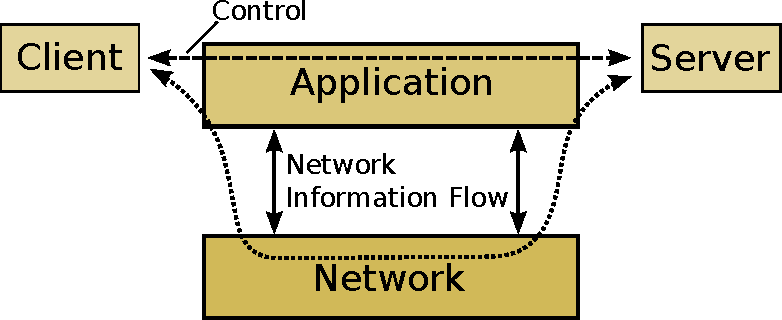
\includegraphics[width=0.8\textwidth]{images/nif.pdf}
\caption{Theoretical information exchange paths between streaming partners.}
\label{c3:fig:nif}
\end{figure}

In every network architecture there is a control information flow between its participating layers, protocols and elements (cf. also Fig. \ref{c3:fig:nif}). Control information may need to be exchanged to coordinate and negotiate the modes of communication between two endpoints and can be helpful in many ways. For example can a network explicitly expose network's quality of service data to applications or these application can make reservation requests to the network. Communication can also work implicitly, demonstrated in the distributed TCP congestion control enabled by the lack of resource isolation. This shows two major ways for the information flow to be implemented: Either through directly and explicitly exchanging information or by one participant implicitly drawing conclusions on another participants resources and behavior.

These different approaches can also be observed in video streaming. The explicit control structure of protocol suites like IMS\cite{3gpp.23.228} and MBMS weaves application and network layer tightly together. This theoretically allows for an improved streaming performance at the cost of universally applicable behavior. Today's IP-based HTTP streaming forms the other side of the pole having only an implicit network information flow by guessing the current network conditions.

For the future there are open questions on how to best incorporate this information flow into streaming applications. Of special interest is the kind of information an application should rely on, and which information the application really requires. Moreover, it is to be decided what and how information should flow in the network. To support the decision making, models and ways to evaluate and compare protocols and network architectures need to be thought out, possibly resulting in a generic evaluation model.

%%%%%%%%%%%%%%%%%%%%%%%%%%%%%%%%%%%%%%%%%%%%%%%%%%%%%%%%%%%%%%%%%%%%%%%%%%%%%%%%
\subsection{Streaming by the Book}
\subsection{RTP}


The established standards for video streaming use combinations of RTP, RTSP, and RTCP \cite{rfc3550, rfc2326}. They are the classic approach to video streaming according to literature (cf., e.g., \cite[p.~589ff]{kurose2008computer}, and \cite[p.~426ff]{peterson2007computer}),  RTP is a dedicated streaming protocol suite, that offers out-of-band control using TCP with separate UDP-based content transport channels. However, the requirement of several open UDP sockets does not work well in environments using middleboxes, .e.g, firewall or network address translation (NAT) nodes, because of the difficulty to forward incoming UDP packets to the destined host. Furthermore, it mandated additional software to be installed at the client. 

RTP streaming is a push-based design. This means, that the server is in control of every aspect of the streaming. When the client requests the start of the playback over the control channel, the server starts pushing down the data over one RTP path. The server application completely controls the transmission speed and the video quality. Therefore, performance and quality metrics have to be exchanged between the two communicating nodes to allow for informed choices on the server side.

RTP also offered intricate multicasting mechanisms, i.e., the ability to simultaneously deliver the same stream to multiple nodes using specially configured routers. These mechanisms were however never fully adopted by the majority of Internet users. On the one hand the required infrastructure was only available in some provider networks, never at the Internet's full scale. On the other hand, the rise of community pages like YouTube has shown, that the interest does not lie in watching the same content at the same time, but rather in high individualism. Therefore, multicast is less relevant for today's streaming. If there is a media event that is streamed live, one can always fall back to using the relatively new structures of Content Delivery Networks (CDN) to be able to serve large groups of users while still conserving bandwidth on the Internet backbones.

There are also other proprietary and standardized streaming systems which better fulfil the requirements of specific fields of applications.  Multimedia Broadcast Multicast Services (MBMS)\cite{3gpp22.146,3gpp22.246} is a specification defined by the 3GPP group for multicasting multimedia traffic specific to the architecture in mobile networks. But similar to RTP the number of implementations and their acceptance are negligible.

%%%%%%%%%%%%%%%%%%%%%%%%%%%%%%%%%%%%%%%%%%%%%%%%%%%%%%%%%%%%%%%%%%%%%%%%%%%%%%%%
%%%%%%%%%%%%%%%%%%%%%%%%%%%%%%%%%%%%%%%%%%%%%%%%%%%%%%%%%%%%%%%%%%%%%%%%%%%%%%%%
%%%%%%%%%%%%%%%%%%%%%%%%%%%%%%%%%%%%%%%%%%%%%%%%%%%%%%%%%%%%%%%%%%%%%%%%%%%%%%%%
\section{Streaming Transport and Clasification}


It can be questioned whether HTTP and TCP are the right choices for transporting media streams.
While there are noteworthy benefits from the features, the ease of use, and the pervasiveness, it was also necessary to resort to application layer flow control to circumvent the lack of direct influence on them.

Through TCP's reliability the whole video file will always be transferred during the streaming process. As mentioned, adverse network conditions can cause TCP's mechanisms to increase latency, jitter as well as reduce the throughput. Protocols that offers congestion control but no reliable delivery and video codecs that are robust to packet loss might be more desirable for streaming. DCCP \cite{kohler2006designing} is an example for such a compromise and might prove beneficial for the streaming process.

HTTP is a state-less request-response protocol. The synchronous behavior of the request-response mechanism does not allow for server events to be sent in a timely manner to the client. This increases the difficulty of implementing some extended features. Examples are server-side load balancing, or real time or live streaming. WebSocket\footnote{\url{http://www.websocket.org/}} \cite{ietf2011websocket} is a protocol running atop of HTTP offering connection multiplexing and asynchronous as well as full duplex communication. It could be used to implement a more flexible HTTP video streaming offering or unlocking further use cases. Similar approaches should be included and evaluated in the research for this thesis.

One future trend is said to be an increase in the required communication confidentiality and authentication. One of the goals might be to enable full end-to-end encryption on the transport level of the network. This could be achieved either by providing an encrypting alternative to TCP, e.g. CurveCP \cite{curvecpwww} and TCPCrypt \cite{tcpcrypt}, or by using HTTPS and moving other functionality further up the stack.


%%%%%%%%%%%%%%%%%%%%%%%%%%%%%%%%%%%%%%%%%%%%%%%%%%%%%%%%%%%%%%%%%%%%%%%%%%%%%%%%
\subsection{UDP-based Techniques}


%%%%%%%%%%%%%%%%%%%%%%%%%%%%%%%%%%%%%%%%%%%%%%%%%%%%%%%%%%%%%%%%%%%%%%%%%%%%%%%%
\subsection{TCP-based Techniques}
\subsubsection{Proprietary}
\subsubsection{,,Simple'' HTML Streaming}
\subsubsection{Adaptive HTML Streaming Techniques}
\subsubsection{\ac{DASH}}


HTTP streaming pursuits a pull-based approach. The client establishes TCP connections to send HTTP requests for video files stored on the Web server, which are then sent to the client. During the sequential downloading process the client can at any time start playing the file even before it is completely downloaded, resulting in a so-called pseudo-streaming behavior.
With this principle the client makes its own decisions regarding the playback process. It has intrinsic knowledge on the current and estimated future connection quality. This leads to a shift of control logic from the server to the client. The former can now be implemented very lightweight, allowing, e.g., for a more distributed content placement in the Internet, especially when using.

By using HTTP the ideal platform for the client is either a plugin living inside a Web browser, the method chosen by Flash, or the browser itself, that in most cases has built-in video playback capabilities.

The capabilities and shortcomings of these novel mechanisms are not yet fully researched making it one of the prime foci of the thesis. Of special interest are:
 
\begin{itemize}

\item \textit{Playback control and media data buffering}. Using the reliable TCP as transport protocol means that there will be no packet loss visible to the application layer. The video file will always reach the client in the same form as stored on the server. If packets are lost, the result will additional delay and decreased throughput through the occurring retransmissions. If video data does not reach the client in time before its playback buffer is depleted, this will results in video stalling and therefore a perceptible loss of quality. This situation can be alleviated or even avoided by carefully planning the playback process and the buffering behavior.

\item \textit{Application layer flow control}. HTTP file downloading is a very simple process. The server has very little influence on this and just forwards requested stored data into a TCP socket. This is not an optimal behavior for video streaming as it does not allow for any throttling or rate management. The buffer space in mobile or embedded devices can be very limited, it would be useful to limit the amount of received data while still ensuring sufficiently available future playback data in the buffer. Services have begun to implement application layer flow control mechanisms for their video streaming application, e.g. YouTube \cite{alcock2011application}. Figure \ref{c3:fig:streamingtransfermodes} shows a comparison of several possible rate management modes. The first sequence diagram shows the unaltered transfer mode observable in regular HTTP file transmissions. The second and third diagrams show possible ways of implementing application layer flow control with either evenly spread out transmissions or sending in blocks. The last diagram displays a mode using multiple requests for one video which can be facilitated for rate adaptations discussed in the next item.

\begin{figure}[htbp]
\centering
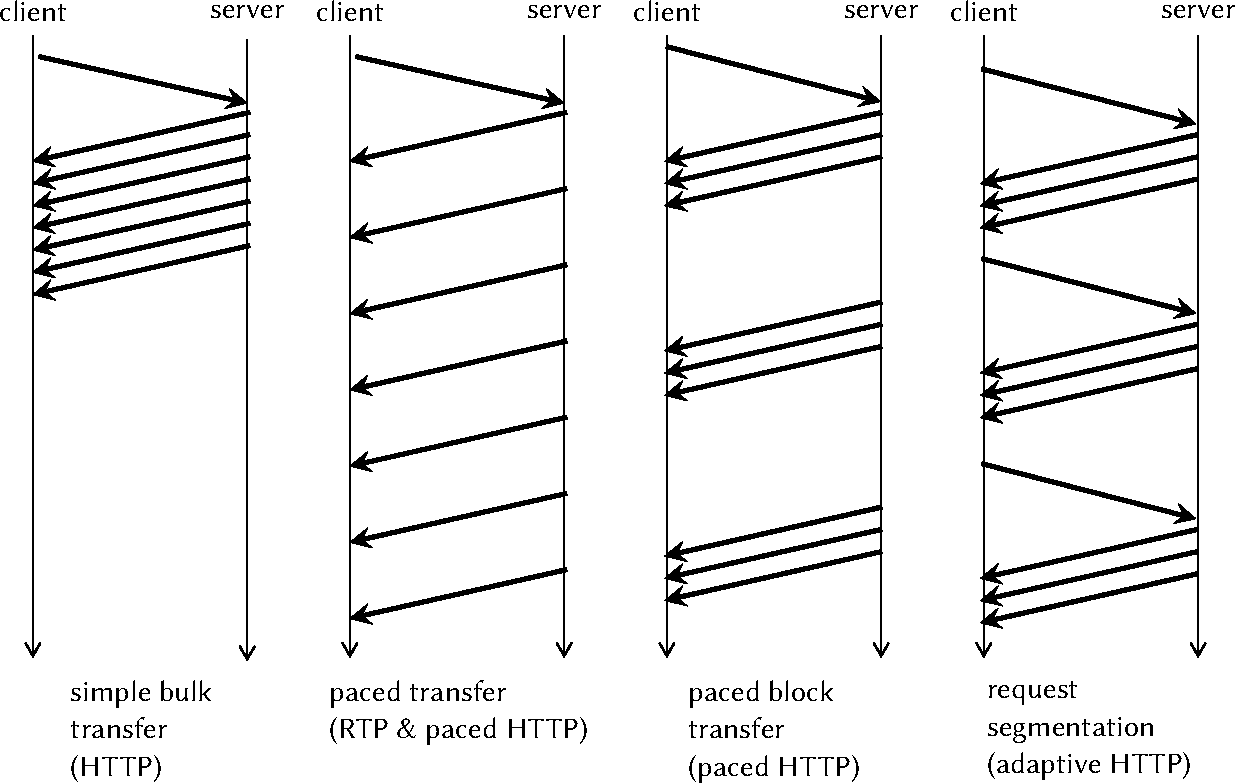
\includegraphics[width=1.0\textwidth]{images/streaming-transfer-modes.pdf}
\caption{Comparison of several possible streaming transfer modes (Source: \cite{ma2011mobile}).}
\label{c3:fig:streamingtransfermodes}
\end{figure}

\item \textit{Video quality and rate adaptation}. To be able to support varying video bitrate levels similar to RTP some adaptations to HTTP streaming are needed. At first, the video has to be encoded multiple times to several output bitrates. Also, the video container needs to be able to support switching the stream at will with everything required for the playback in place. Additionally, an independently available index file needs to correlate the video files with their contents. Alternatively, the video can be segmented into short pieces of several seconds outlined by a separate index file. Then the client can choose the stream variant that best fits its current condition, which depends on parameters including the display size or varying network QoS. \cite{ma2011mobile} gives an overview over some possibilities. Several proprietary protocols, some of them in the process of standardization, tackle this, including HTTP Live Streaming \cite{pantos2011livestreaming} and Microsoft Smooth Streaming \cite{zambelli_iis_2009}. They are either based on file segmentation or HTTP RANGE requests. Initial experiments in \cite{akhshabi2011experimental} evaluate the viability of this kind of approach. We plan to extend this by modelling the fundamental building blocks the mechanisms have in common and after that giving tools to find and evaluate combinations best suited to specific network conditions.
This includes evaluations of the optimal length of segments as well as tuning the aforementioned buffering models to be able to cope with at least two new degrees of freedom, i.e. being able to load multiple segments at once using more than one connection as well as the ability to switch to another video encoding level in case of changing connection capacity or buffer pressure conditions.

\end{itemize}

The focus of the thesis will be to explore the possibility space of the aforementioned mechanisms and give the ability to make informed choices on the viability of them or whole protocols for specific use cases.



%%%%%%%%%%%%%%%%%%%%%%%%%%%%%%%%%%%%%%%%%%%%%%%%%%%%%%%%%%%%%%%%%%%%%%%%%%%%%%%%
\subsection{Features of HTTP Streaming}

The leitmotif of HTTP streaming is the inversion of control compared to RTP streaming. Due to UDP's lack of reliability, congestion control, and flow control features, RTP does need to do this on its own. Therefore, the RTP server application is responsible to implement and conduct these, increasing its complexity. Even playback control is done by the server, albeit at the request of the client. Web-streaming turns this around and puts the client in charge. Because HTTP streaming relies on TCP explicit server control is unnecessary. Control is now done either implicitly by the transport protocol or explicitly by the client, e.g. playback control which also plays an important role in buffer management. This inversion also eliminates the need to exchange client metrics to the server, but increases the complexity of the client. Moreover, TCP's reliable transport feature may prove to negatively affect playback in suboptimal network conditions.

%Because HTTP streaming relies on TCP this is not necessary, but it also removes a bit of flexibility, as the type of congestion control is given. 


In its simplest form Web streaming acts like regular HTTP traffic. The video is requested and then delivered from the server in one single block transfer. The transfer is controlled by the server and it can employ pacing mechanisms to somewhat match the download duration to the playback duration. This reduces load spikes and the required buffer size on the client device but also makes the process more vulnerable to changing network conditions. YouTube uses a server-side pacing mechanism which is  discovered in \cite{alcock2011afcyt}\footnote{\url{http://www.wand.net.nz/~salcock/youtube/}} and also discussed in Section \ref{c3:sec:measurements}.

These simple mechanisms, however, can not seamlessly change quality in a currently running video. This can be important for, e.g., mobile networks or when an increasingly loaded server can not fulfill every request in its highest quality at the required speed anymore.

Therefore adaptive forms of HTTP streaming were developed. The techniques complement and extend the server-side pacing mechanisms and introduce video quality and bitrate adaption to HTTP streaming by doing file segmentation \cite{ma2011mobile, watching-video1}. Bitrate adaption, belonging to a class of application-layer flow control mechanisms, can add an extra level of feedback to react to changing network conditions but could also make buffer management more complex. Protocols based on this approach are already widespread, e.g. in Netflix's offerings.



%%%%%%%%%%%%%%%%%%%%%%%%%%%%%%%%%%%%%%%%%%%%%%%%%%%%%%%%%%%%%%%%%%%%%%%%%%%%%%%%
\subsection{Proprietary Approaches}






%%%%%%%%%%%%%%%%%%%%%%%%%%%%%%%%%%%%%%%%%%%%%%%%%%%%%%%%%%%%%%%%%%%%%%%%%%%%%%%%
\subsection{Network Stack Layers and Streaming}
\label{sec:analysis}

In network layering models, it is often assumed that the layers are independent (or at least strongly decoupled) from, and only present narrow interfaces to, one another. From a conceptual point of view, media streaming is a process governing the application layer. Thus, the application and its behavior might be thought to dominate the overall streaming process and associated quality. In this Section, we will show that this is not necessarily the case. % for reasons of conflicting time constraints on the different layers, 


Figure \ref{c3:fig:timescales} overviews the approximate time scales on which activities on different layers may take place, spanning a remarkable range of twelve orders of magnitude. Multiple layers might implement the same or similar functionality, e.g. flow control in the application and on transport layer, resulting in nested control loops, which might be coupled due to the timing constraints. 


% As such, the aim of this deliverable is to provide a methodology that identifies influencing factors on the user experience, and quantifies the relative impact of these factors.


\begin{figure}[htbp]
	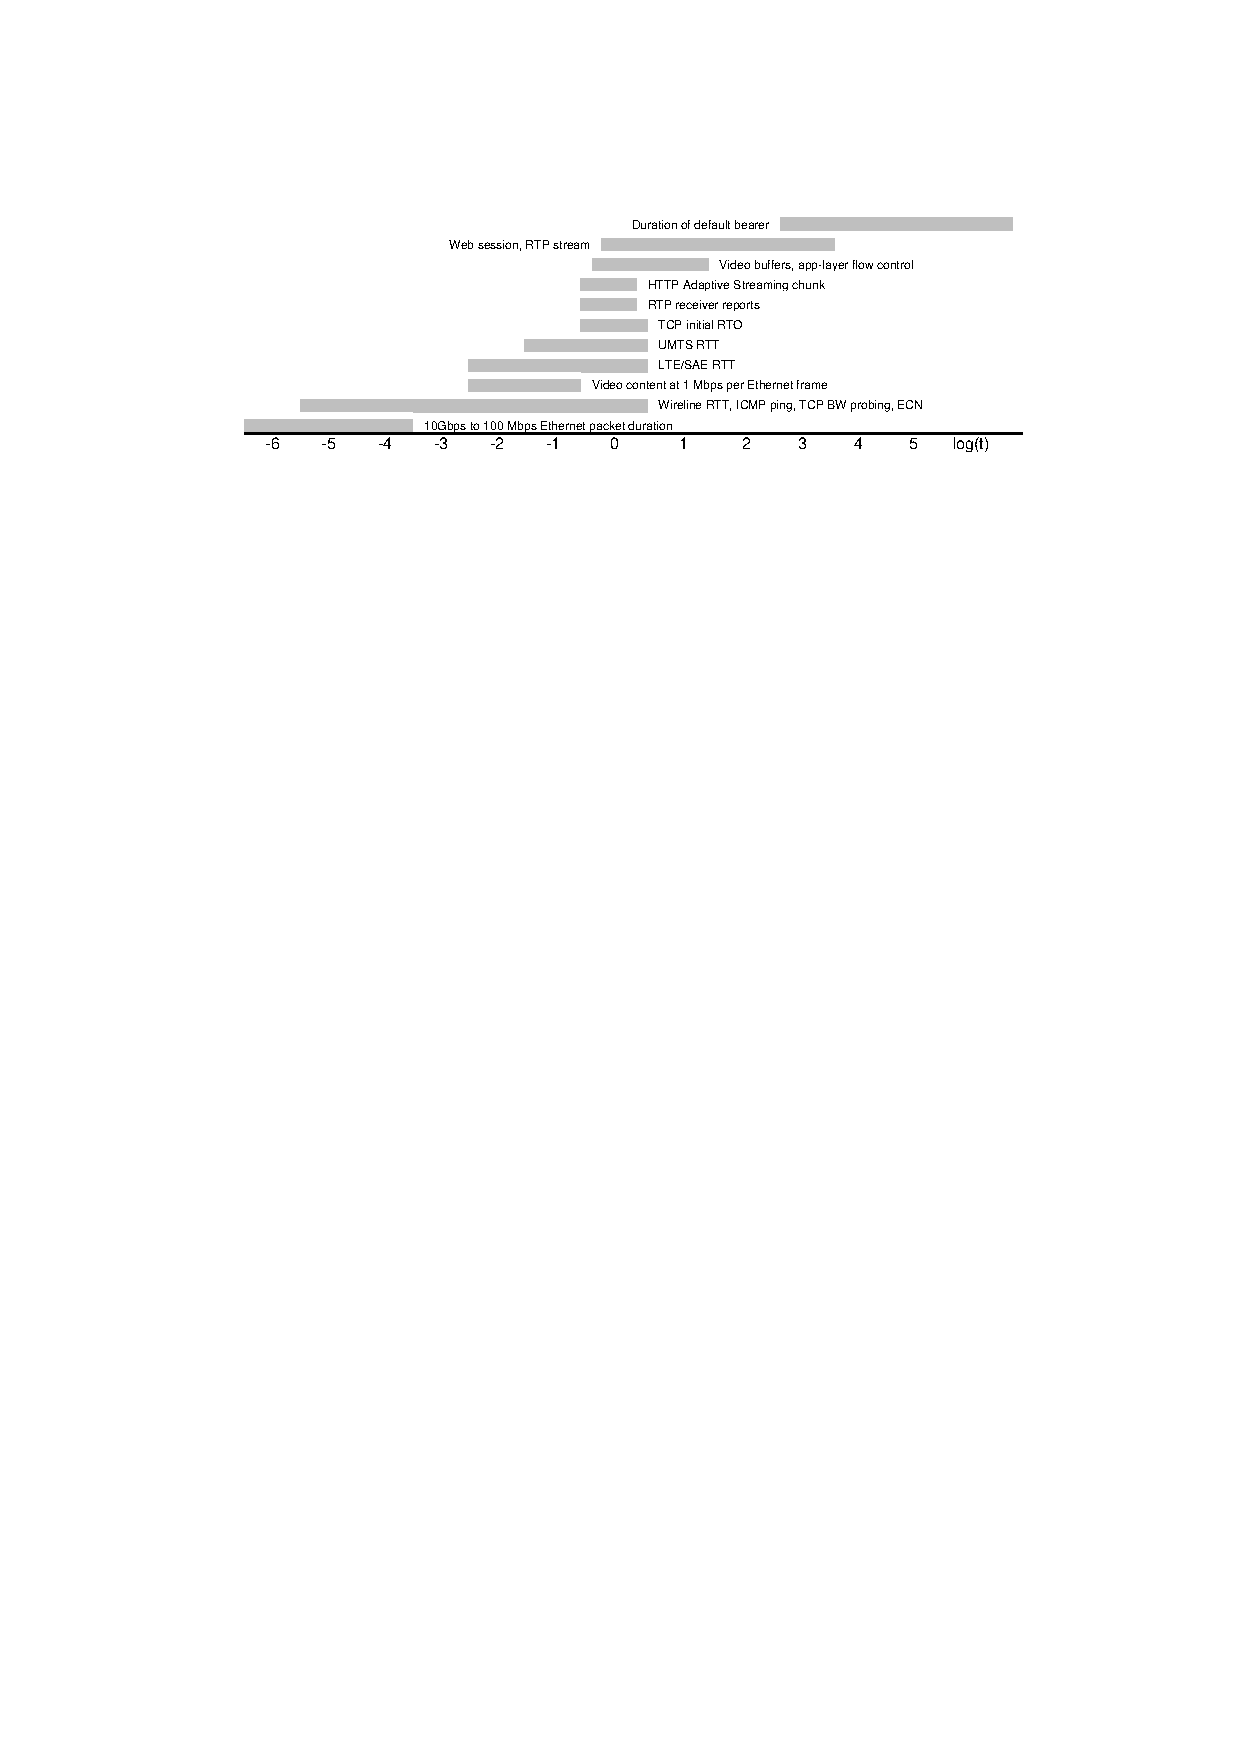
\includegraphics[width=\textwidth]{images/timescales.pdf}
	\caption{Relevant time scales in the layers of the stack}
	\label{c3:fig:timescales}
\end{figure}



\subsubsection{Network Layer}

As seen in Figure \ref{c3:fig:timescales}, the time constants found in different network implementations range from nanoseconds (for Gigabit Ethernet) to seconds (for UMTS and LTE/SAE wireless networks), depending on the technology used. This also influences the achievable round-trip time across such networks, which directly affects the performance of higher-layer protocols: IP, ICMP, UDP, TCP, and subsequently all application-layer protocols are all subject to these timing constraints.

In the case of wireless networks, typical effects of wireless connectivity relating to physical phenomena like fading and interference come into play. Flaky radio connectivity is a major source of packet loss and excessive delay. Certain cellular mobile technologies like UMTS and its evolutions implement loss concealment themselves, confounding IP's assumption of a host-to-network layer lacking guaranteed delivery. Other peculiarities of cellular mobile networks include a maximum transmission unit (MTU) opaque to IP, and delay variances as functions of packet sizes \cite{Arlos10} and radio access technologies \cite{laner2011dissecting}.


% Then, the technological progress enables both handsets and the network to become faster: Compar-ing the delay budgets given by [ANDE] for UMTS (2005) and [KESS] for HSDPA R99 (2009) respectively, it is seen that the delay caused by pro-cessing on the mobile terminals decreased by a factor of 30, and that the core network has become faster by an order of magnitude as well. [SVOB] has additional information on the delay budgets per network entity, varying the packet size as the parameter.
%LTE/SAE also makes heavy use of the concept of bearers, a type of tunnel through the mobile network associated with quality levels and policy control. Although the bearer concept already exists in UMTS, operators seem cau-tious to configure other bearers than the default one, and support by hand-sets is not widespread either. The process of setting up LTE bearers is specified amongst others in [3GP23]. The setup procedure is sufficiently lengthy to be measurable and influence packet delay on initiating connec-tions [FIED]. Analyzing the effects of bearers on user data flows is the sub-ject of the Ursa Major project [URSA] at the University of Vienna with the FTW.
%
%For reasons of radio spectrum efficiency, applications with long patterns of inactivity may be scheduled to not use HSDPA. This also causes measura-ble additional delay for applications [SVOB and their references 3 and 4].
%


\subsubsection{Transport Layer}

%As detailed in Section 3, the application and associated application-layer protocols dictate certain requirements on the transport protocol to be used.

The two most widely used transport protocols are TCP (Transmission Control Protocol) and UDP (User Datagram Protocol). As is widely known, TCP implements a number of elaborate mechanisms to establish and tear down connections, deliver data to the application in sequential order, conceal loss on the network layer, adapt its bandwidth usage to the capabilities of the other endpoint (flow control) and the network (congestion control), and share bandwidth fairly through a distributed control algorithm. Furthermore, its notion of ports adds a layer of addresses on top of the network layer.

UDP also supports port numbers, but does not include any of the other mechanisms TCP has. This spurs the common misconception that UDP is the faster transport protocol. In fact, all packet types are subject to the same round-trip time, independent of the transport protocol used. Delays in the delivery of data to the upper layer occur in TCP when segments are considered lost in transmission (via timeouts or gaps in the range of acknowledged segments). TCP retransmits the lost segments, causing the round-trip time to spike temporarily. In the case of UDP, the application layer handles (or ignores) packet loss.

As indicated in the previously, mobile cellular networks often conceal packet loss, which is used by TCP as an indication for network congestion. Rather than lost, packets are highly delayed, which can cause sub-optimal bandwidth usage. Mobile networks also show artifacts relating to port and network address translation (commonly subsumed under ``NAT''), firewalling, and middleboxes interfering with TCP timeout on long-lived connections \cite{wang2011untold}.


%It must be noted that the loss of acknowledgements can usually not be discriminated from actual packet loss, and 
%
%nor does its assumption of loss hold in the face of highly varying delays, i.e. jitter, as typically found in mobile networks.

%There are lots of controls for mobile operators to engineer traffic flows in their networks. In \cite{wang2011untold}, the authors show artifacts relating to port and network address translation (commonly subsumed under “NAT”), firewalling, IP address assignment etc. Operators can also employ traffic engineering on backhaul links, and use policies to better support (or regulate) specific services for specific users or user groups, schedule traffic at different times of the day, etc.



\subsubsection{Application Layer}

There exists a diversity of streaming applications and associated application-layer protocols, each supporting to differing degrees certain types of streaming, and each having its own set of requirements, depending on the content type (pre-generated or live), the codec and its bitrate, and playback control and quality feedback.

One classification for streaming protocols might be their body of standardization: There are many proprietary protocols with undisclosed or legally restricted standards documents, e.g. RTMP (Real Time Messaging Protocol) and RTMPCS (RTMP Chunk Stream), MMS (Microsoft Media Server), and WMSP (Windows Media HTTP Streaming Protocol). Other protocols and protocol families are standardized by open bodies such as the Internet Engineering Task Force (IETF). In our work, we focus on these ``open'' protocols.

In the latter category are two well-known protocol families for media streaming, Real-time Transport Protocol (RTP) and Hypertext Transfer Protocol (HTTP). RTP sees most of its use in walled garden services such as IP TV. HTTP is the single most common application layer protocol on the Internet, owing its popularity to the ubiquity of web browsers. As RTP is designed for media transport, a companion protocol suite consisting of RTCP (for control information), RTSP (for stream control like pausing), and SDP (for session management) is often used. RTP is mostly transported using UDP.

In contrast to RTP, HTTP was not designed for specific payload types apart from HTML. The actual streaming protocol behavior is defined by the application, not by the protocol. Every service is thus free to define its own distinct protocol behavior. For HTTP, many de-facto variants for streaming exist, but many if not most are not formally standardized. There is work underway in the IETF to create a standard for Dynamic Adaptive Streaming over HTTP (DASH).



Within these protocol families, a multitude of implementations exist that suit specific demands. RTP specifies an initial set of profiles (RFC3551), with a multitude of definitions cropping up with every new type of media coding scheme . In HTTP, the actual transfer model, addressing, and metadata mechanisms have been in place virtually unchanged since 1999, when HTTP/1.1 was specified. Much innovation has since gone into the payloads transferred via HTTP, as well as the control of its underlying transport protocol, TCP.

Both protocol families offer a wide range of techniques, established and recent, de-facto and formally standardized, each supporting different types of streaming and content, and each subject to the interplay of content requirements, the application, the network, the media player, the layer stack, etc. Seemingly, not one single protocol can solve all problems at once. % Let’s now look at the specific properties of RTP and HTTP.


The Real-time Transport Protocol (RTP) [RFC3550] is an IETF protocol designed for (near) real-time payload such as multimedia or sensor data. It is designed for support by the network. RTP supports mixers and translators that enable transcoding of content as it travels through the network.

Since RTP is typically transported over UDP, it is also multi-cast compatible. For example, A1 Telekom Austria’s A1 TV uses an Organization-local cope Multi-cast [RFC2365] tree with distinct IP addresses for each program. At the same time, UDP is not inherently congestion-controlled, and RTP’s own congestion control mechanism (if activated at all) has a relatively long delay to respond for reasons of rate limiting on the control channel (see [RFC3550, Sec. 3.5.1] for details). This means a wide-spread use of RTP could even cause congestion collapses in parts of the network.

RTP employs a server-side control scheme. This means that the server is responsible for every aspect of the streaming process. Even client play and pause requests are directly communicated to the server. Therefore the server also has to maintain a session for the user.



In contrast to RTP, HTTP streaming facilitates complete client side control. HTTP includes some support by the network in the form of proxies, but there are signaling methods that can e.g. forbid the caching of specific content through the no-cache directive [RFC2616, Sec. 14.9.1].
Due to its use of TCP as the transport protocol, HTTP has issues with inter-activity, especially across lossy links.
3.2	Protocol Comparison
In Figure 3, we compare the properties of three specific implementations of streaming protocols, namely RTP with RTCP, progressive HTTP, and adaptive HTTP. In RTP streaming, it is customary to have multiple flows for different parts of the media stream, e.g. audio and video, and a separate control connection. In HTTP, one (or multiple consecutive) TCP connection is used for both control and data transfer.
In RTP, flow control on the transport layer needs to be done by the server application. The same goes for congestion control, which is implemented us-ing receiver reports, or might be left out altogether. HTTP uses TCP as its transport protocol, and thus inherits its flow control and congestion control features.
There are several implementations for application-layer flow control. Figure 4 shows an overview on basic and modern flavors. Simple bulk transport is the typical web download model, which assumes that both the client and the server try to transfer the data as fast as possible. Contrarily, paced transfer is implemented by RTP, where the server sets the bitrate the client will see. An interesting variant on paced transfer is paced block transfer, implement-ed for example in the YouTube block sending mechanism [METZ]. The specific incarnation consists of server-controlled burst sending of 64kB blocks and inter-block gaps of variable length to adjust the download rate to the average video bitrate. An additional initial burst phase is present to prefill buffer. The method is observed in detail in [ALNE11].
 
Playback control is actually done by the server in the case of RTP, where the client issues requests to, e.g., pause the stream, and the server then reacts. In HTTP, the client is in much stronger control of the playback, and need not notify the server of a user’s decision to skip backwards, etc. 
For the exchange of transport control information such as packet loss, RTP uses a companion protocol named Real-Time Control Protocol (RTCP). HTTP again leverages TCP, where such information is exchanged implicitly. It must be noted however that due to the flexible data format RTCP pro-vides, more concise information can be signaled in addition to transport control related matters.
To conclude, the different protocols are also specified to different degrees. As stated before, there is a large body of RFCs relating to RTP and its adaption to new media, content, etc. For HTTP, many de-facto used variants adapted to streaming exist, but many if not most are not formally standardized. There is work underway in the IETF to create a standard for Dynamic Adaptive Streaming over HTTP (DASH) .








